The general equation of a second degree can be expressed as,
\begin{align}
\vec{x^T}\vec{V}\vec{x} + 2\vec{u^T}\vec{x} + f = 0 \label{eq:solutions/4/2/11eq:3}
\end{align}
Comparing \eqref{eq:solutions/4/2/11eq:2} and \eqref{eq:solutions/4/2/11eq:3} we get,
\begin{align}
\vec{u} = \myvec{-4 \\ -3} \label{eq:solutions/4/2/11eq:4}
\end{align}
\begin{align}
f = 7 \label{eq:solutions/4/2/11eq:5}    
\end{align}
If $\vec{n}$ is the normal vector, $\vec{P}$ is a point on that line then equation of the line can be written as,
\begin{align}
\vec{n^T}\brak{\vec{x-P}} = 0\\
\implies \vec{n^Tx} = c \label{eq:solutions/4/2/11eq:7}
\end{align}
 where c = $\vec{n^TP}$.
Comparing \eqref{eq:solutions/4/2/11eq:1} and \eqref{eq:solutions/4/2/11eq:7} we get,
\begin{align}
\vec{n} = \myvec{1 \\ 1} and \ c = 1 \label{eq:solutions/4/2/11eq:8}
\end{align}\\
The point of contact q, of a line with a normal vector $\vec{n}$ to the conic in \eqref{eq:solutions/4/2/11eq:3} is given by,
\begin{align}
\vec{q} = \vec{V^{-1}}\brak{\kappa\vec{n} - \vec{u}} \label{eq:solutions/4/2/11eq:9}
\end{align}
\begin{align}
\kappa = \pm \sqrt{\frac{\vec{u^TV^{-1}u}-f}{\vec{n^TV^{-1}n}}} \label{eq:solutions/4/2/11eq:10}
\end{align}\\
For a circle,
\begin{align}
\vec{V} = \vec{I} \label{eq:solutions/4/2/11eq:11}
\end{align}
where I is the Identity matrix..
Solving for $\kappa$ using \eqref{eq:solutions/4/2/11eq:10} we get,
\begin{align}
\kappa = \pm 3 \label{eq:solutions/4/2/11eq:12}
\end{align}
\begin{align}
i.e. \ \vec{q_1} = \myvec{1 \\ 0} \ for \ \kappa = -3 \label{eq:solutions/4/2/11eq:13}
\end{align}
and
\begin{align}
\vec{q_2} = \myvec{7 \\ 6} \ for \ \kappa = 3 \label{eq:solutions/4/2/11eq:14}
\end{align}
To prove that the line touches the circle at $\vec{q}$ need to check that
\begin{align}
\vec{m^T}\brak{\vec{V}\vec{q}+\vec{u}} = 0 \label{eq:solutions/4/2/11eq:15}
\end{align}
We know that,
\begin{align}
\vec{m^T}\vec{n} = 0 \label{eq:solutions/4/2/11eq:16}
\end{align}
\begin{align}
\implies m = \myvec{$-$1 \\ 1} \label{eq:solutions/4/2/11eq:17} 
\end{align}\\
Using \eqref{eq:solutions/4/2/11eq:13}, \eqref{eq:solutions/4/2/11eq:14} and \eqref{eq:solutions/4/2/11eq:17}, the expression in \eqref{eq:solutions/4/2/11eq:15} holds true for both $\vec{q_1}$ and $\vec{q_2}$ which means that both those points lie on the circle i.e. there will be a tangent passing through each of them which can be found out using \eqref{eq:solutions/4/2/11eq:7}
\begin{align}
i.e. \ \vec{n^T}\vec{q_1} = c_1 \label{eq:solutions/4/2/11eq:18}
\end{align}
\begin{align}
\vec{n^T}\vec{q_2} = c_2 \label{eq:solutions/4/2/11eq:19}
\end{align}
where,
\begin{align}
c_1 = \vec{n^Tq_1} = \myvec{1 & 1}\myvec{1 \\ 0} = 1  \label{eq:solutions/4/2/11eq:20}
\end{align}
which was already obtained in \eqref{eq:solutions/4/2/11eq:8} and\\
\begin{align}
c_2 = \vec{n^Tq_2} = \myvec{1 & 1}\myvec{7 \\ 6} = 13 \label{eq:solutions/4/2/11eq:21}
\end{align}
Using \eqref{eq:solutions/4/2/11eq:18} the given line in the question is obtained which is \eqref{eq:solutions/4/2/11eq:1}.
Therefore, the tangent parallel to \eqref{eq:solutions/4/2/11eq:1} is,
\begin{align}
\myvec{1 & 1}\vec{x} = 13 \label{eq:solutions/4/2/11eq:22}
\end{align}\\
And the line(s) perpendicular to \eqref{eq:solutions/4/2/11eq:1} can be found out using \eqref{eq:solutions/4/2/11eq:8} and here the normal vector for this line will be $\vec{m}$ which was calculated using \eqref{eq:solutions/4/2/11eq:17} and its equation(s) will be,
\begin{align}
    \vec{m^Tx} = c_3 \label{eq:solutions/4/2/11eq:23}
\end{align}
\begin{align}
    \vec{m^Tx} = c_4 \label{eq:solutions/4/2/11eq:24}
\end{align}
where,
\begin{align}
c_3 = \vec{m^Tq_1} = \myvec{-1 & 1}\myvec{1 \\ 0} = -1 \label{eq:solutions/4/2/11eq:25}
\end{align}
\begin{align}
c_4 = \vec{m^Tq_2} =  \myvec{-1 & 1}\myvec{7 \\ 6} = -1  \label{eq:solutions/4/2/11eq:26}
\end{align}\\
Therefore, the line perpendicular to \eqref{eq:solutions/4/2/11eq:1} and also to \eqref{eq:solutions/4/2/11eq:22} is,
\begin{align}
 \myvec{-1 & 1}\vec{x} = -1 \label{eq:solutions/4/2/11eq:27}   
\end{align}

In Fig. \ref{eq:solutions/4/2/11Fig.1}. $\vec{C}$ is the center of the circle. $\vec{q_1}$ and $\vec{q_2}$ are points of contact with the circle. 
\begin{figure}[!ht]
\centering
    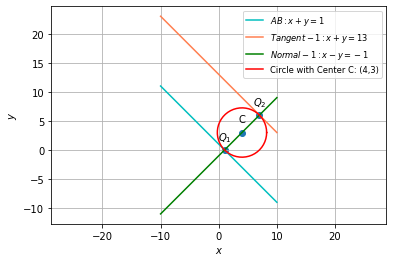
\includegraphics[width=\columnwidth]{./solutions/4/2/11/Figure.png}
    \caption{Tangents and Normal on the Circle}
    \label{eq:solutions/4/2/11Fig.1}
\end{figure}
\\
Line 1 is \eqref{eq:solutions/4/2/11eq:1}, Line 2 is \eqref{eq:solutions/4/2/11eq:22} and Line 3 is \eqref{eq:solutions/4/2/11eq:27}.
